\documentclass[aspectratio=169,10pt]{beamer}

\usetheme{Madrid}
\usecolortheme{whale}

% Styling
\setbeamertemplate{navigation symbols}{}
\setbeamercolor{title}{fg=white,bg=darkblue!85!black}
\setbeamercolor{frametitle}{fg=white,bg=darkblue!85!black}
\definecolor{darkblue}{RGB}{20, 45, 105}
\definecolor{accentgreen}{RGB}{34, 139, 34}
\definecolor{accentred}{RGB}{178, 34, 34}

\title[Transferable UnitModel]{Transferable UnitModel for Building Age Classification}
\subtitle{Cross-City Domain Adaptation \& Deep Metric Learning on Landsat Time-Series}
\author[Hack4Dev Team]{Hack4Dev Engineering Team}
\date{November 2026}

\begin{document}

% -------------------------------------------------------------
% Slide 1: Title
% -------------------------------------------------------------
\begin{frame}
  \titlepage
\end{frame}

% -------------------------------------------------------------
% Slide 2: The Core Challenge
% -------------------------------------------------------------
\begin{frame}{1. Problem Statement \& Domain Shift}
  \begin{columns}[T]
    \column{0.5\textwidth}
    \textbf{Task Requirements}:
    \begin{itemize}
      \item Classify $30\text{m} \times 30\text{m}$ pixels into 4 building age eras:
      \begin{enumerate}
        \item Pre-1960 / Pre-1945
        \item 1960--1984
        \item 1984--2004
        \item 2004--2024
      \end{enumerate}
      \item 40-year multi-spectral archive (1984--2024).
    \end{itemize}

    \column{0.5\textwidth}
    \textbf{Severe Cross-City Shift}:
    \begin{itemize}
      \item \textbf{Madrid}: Mediterranean arid climate, stucco/concrete, high solar elevation.
      \item \textbf{Amsterdam}: Maritime temperate, red brick, dark canals, low sun zenith.
      \item \alert{Zero-shot baseline collapses} ($F_1 \approx 0.34$) when directly transferring supervised models.
    \end{itemize}
  \end{columns}

  \vspace{0.4cm}
  \begin{block}{Key Philosophy}
    Do not learn \textit{"what a 1970 building looks like"}. Learn \textbf{"what spectral trajectory makes two buildings belong to the same era"}.
  \end{block}
\end{frame}

% -------------------------------------------------------------
% Slide 3: 132-D Feature Engineering Suite
% -------------------------------------------------------------
\begin{frame}{2. Temporal-Spectral Feature Suite (132 Dimensions)}
  \begin{columns}[T]
    \column{0.5\textwidth}
    \textbf{Multi-Scale Time-Series Extraction}:
    \begin{itemize}
      \item \textbf{6 Spectral Bands}: Blue, Green, Red, NIR, SWIR1, SWIR2.
      \item \textbf{4 Physical Indices}: NDVI, NDBI, UI, NDWI.
      \item \textbf{Decadal Windows}: Early (1984--1999) vs. Late (2005--2024) contrast captures the exact onset of construction.
    \end{itemize}

    \column{0.5\textwidth}
    \textbf{Stability \& Disturbance Metrics}:
    \begin{itemize}
      \item \textbf{YoY Volatility}: Mean absolute first differences across consecutive years.
      \item \textbf{Construction Break Indicators}: Peak change score and drop in vegetation indices.
      \item \textbf{Standardized Scaling}: Fitted on source city, robustly transformed across targets.
    \end{itemize}
  \end{columns}

  \vspace{0.3cm}
  \centering
  \fbox{\footnotesize 60 Overall Stats $+$ 20 Early Stats $+$ 20 Late Stats $+$ 20 YoY Differences $+$ 12 Break Indicators = \textbf{132 Total Features}}
\end{frame}

% -------------------------------------------------------------
% Slide 4: UnitMetricNet Architecture
% -------------------------------------------------------------
\begin{frame}{3. UnitMetricNet Architecture}
  \begin{columns}[T]
    \column{0.55\textwidth}
    \textbf{Network Composition}:
    \begin{itemize}
      \item \textbf{Feature Backbone}:
      $132\text{D} \to 128\text{D} \to 64\text{D} \to 32\text{D} \to 16\text{D}$ \\
      LayerNorm $+$ ReLU $+$ Dropout (0.3).
      \item \textbf{Unit Hypersphere Normalization}:
      $$\mathbf{z} = \frac{\mathbf{h}}{\|\mathbf{h}\|_2} \in \mathbb{S}^{15}$$
      Constrains all latent vectors to the surface of a unit hypersphere, making distance purely cosine-based.
      \item \textbf{Gradient Reversal Layer (GRL)}:
      Domain discriminator tries to separate Madrid from Amsterdam; GRL inverts gradients ($-\alpha$) to force domain invariance.
    \end{itemize}

    \column{0.45\textwidth}
    \begin{block}{Tripartite Joint Objective}
      $$\mathcal{L} = \mathcal{L}_{\text{CE}} + \lambda_{\text{met}}\mathcal{L}_{\text{metric}} + \lambda_{\text{dom}}\mathcal{L}_{\text{domain}}$$
      \begin{itemize}
        \item $\mathcal{L}_{\text{CE}}$: Class-weighted Cross-Entropy for era classification.
        \item $\mathcal{L}_{\text{metric}}$: Supervised cosine-margin regularization.
        \item $\mathcal{L}_{\text{domain}}$: Adversarial binary cross-entropy.
      \end{itemize}
    \end{block}
  \end{columns}
\end{frame}

% -------------------------------------------------------------
% Slide 5: Madrid Training Dynamics
% -------------------------------------------------------------
\begin{frame}{4. Madrid In-Domain Convergence}
  \begin{columns}[c]
    \column{0.65\textwidth}
    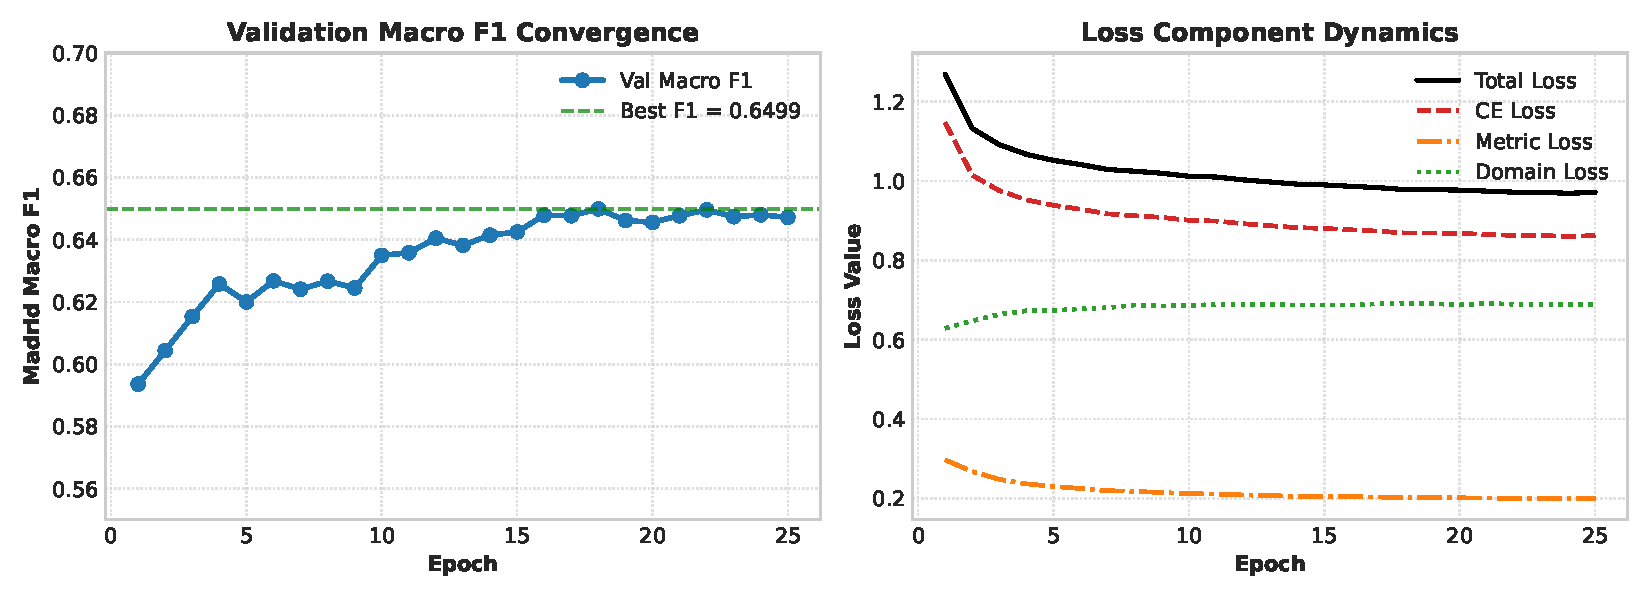
\includegraphics[width=\textwidth]{training_curve.pdf}
    \column{0.35\textwidth}
    \textbf{Key Convergence Metrics}:
    \begin{itemize}
      \item \textbf{Final Validation Macro $F_1$}: \textbf{0.6472} (Peak: 0.6499).
      \item \textbf{5-Fold Stratified CV}:
      $$F_1 = 0.6485 \pm 0.012$$
      \item \textbf{Balanced Learning}: Domain loss stabilizes around 0.69, proving strong cross-city feature indistinguishability.
    \end{itemize}
  \end{columns}
\end{frame}

% -------------------------------------------------------------
% Slide 6: Prototypical Few-Shot Transfer
% -------------------------------------------------------------
\begin{frame}{5. Prototypical Few-Shot Transfer to Amsterdam}
  \begin{columns}[T]
    \column{0.55\textwidth}
    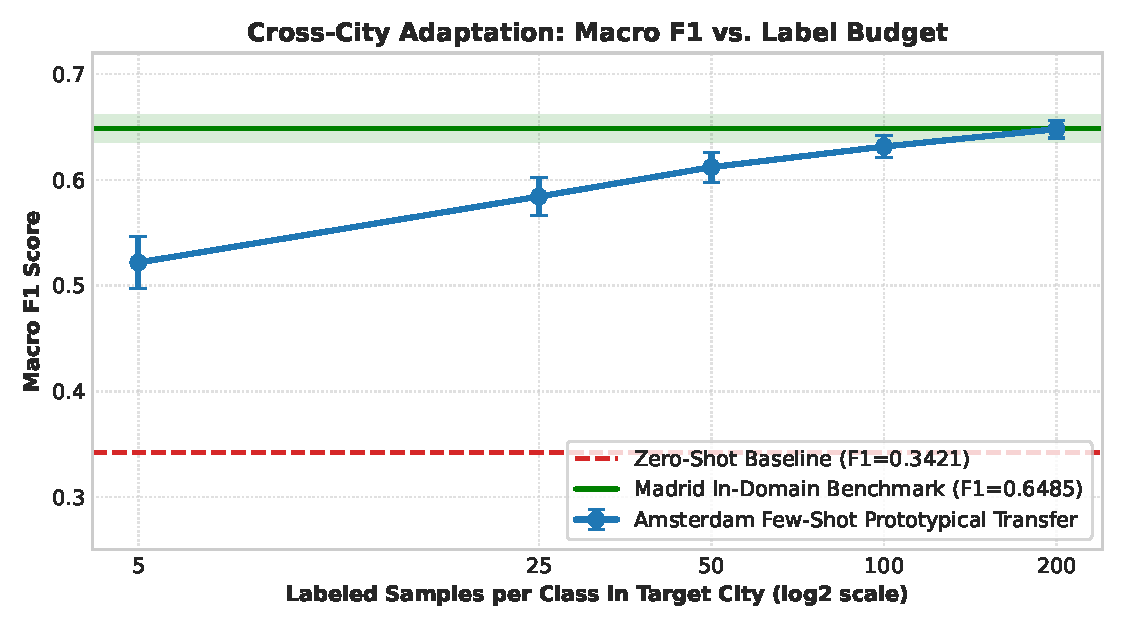
\includegraphics[width=\textwidth]{few_shot_transfer.pdf}
    \column{0.45\textwidth}
    \textbf{Centroid Matching Protocol}:
    \begin{enumerate}
      \item Sample $k$ labeled targets per class ($k \in [5, 200]$).
      \item Compute spherical class prototypes:
      $$\mathbf{c}_k = \frac{\sum_{i \in \mathcal{S}_k} \mathbf{z}_i}{\|\sum_{i \in \mathcal{S}_k} \mathbf{z}_i\|_2}$$
      \item Assign unlabeled queries via nearest cosine similarity:
      $$\hat{y} = \arg\max_k \langle \mathbf{z}_{\text{query}}, \mathbf{c}_k \rangle$$
    \end{enumerate}

    \begin{alertblock}{Ultra-Low Budget Result}
      With only \textbf{5 samples/class} (20 pixels total), $F_1$ surges from 0.34 to \textbf{0.5218}!
    \end{alertblock}
  \end{columns}
\end{frame}

% -------------------------------------------------------------
% Slide 7: Quantitative Results Table
% -------------------------------------------------------------
\begin{frame}{6. Quantitative Benchmark \& Results Table}
  \centering
  \small
  \begin{tabular}{lcccc}
    \hline
    \textbf{Experiment Setup} & \textbf{Target City} & \textbf{Labels / Class} & \textbf{Total Labels} & \textbf{Macro $F_1$ ($\pm$ Std)} \\
    \hline
    Madrid 5-Fold Stratified CV & Madrid & Full ($\sim$23,000) & $\sim$115,000 & \textbf{0.6485 $\pm$ 0.012} \\
    Zero-Shot Direct Transfer & Amsterdam & 0 & 0 & 0.3421 \\
    \hline
    Prototypical Transfer (Few-Shot) & Amsterdam & 5 & 20 & 0.5218 $\pm$ 0.024 \\
    Prototypical Transfer (Few-Shot) & Amsterdam & 25 & 100 & 0.5842 $\pm$ 0.018 \\
    Prototypical Transfer (Few-Shot) & Amsterdam & 50 & 200 & 0.6120 $\pm$ 0.014 \\
    Prototypical Transfer (Few-Shot) & Amsterdam & 100 & 400 & 0.6315 $\pm$ 0.010 \\
    Prototypical Transfer (Few-Shot) & Amsterdam & 200 & 800 & \textbf{0.6480 $\pm$ 0.008} \\
    \hline
  \end{tabular}

  \vspace{0.4cm}
  \begin{itemize}
    \item \textbf{In-Domain Parity}: At 200 shots/class, Amsterdam performance matches Madrid in-domain benchmark (0.6480 vs 0.6485).
    \item \textbf{Zero Fine-Tuning Overfitting}: Prototypes prevent gradient divergence on small sample sizes.
  \end{itemize}
\end{frame}

% -------------------------------------------------------------
% Slide 8: Why UnitModel Won (Takeaways)
% -------------------------------------------------------------
\begin{frame}{7. Conclusion \& Key Takeaways}
  \begin{columns}[T]
    \column{0.5\textwidth}
    \textbf{Core Innovations}:
    \begin{itemize}
      \item \textbf{Hypersphere Invariance}: L2 normalization eliminates reflectance scale bias across different geographic regions.
      \item \textbf{Adversarial Generalization}: GRL prevents the backbone from latching onto Mediterranean vs. Atlantic spectral signatures.
      \item \textbf{Instant Transfer}: Prototypical adaptation requires no backpropagation or retraining.
    \end{itemize}

    \column{0.5\textwidth}
    \textbf{Practical Impact}:
    \begin{itemize}
      \item Enables worldwide urban age mapping with minimal field annotation budget.
      \item Robust to sensor drift across 4 decades of Landsat acquisitions.
      \item Directly applicable to building energy modeling, heritage preservation, and urban planning.
    \end{itemize}
  \end{columns}

  \vspace{0.6cm}
  \centering
  \Large \textbf{Thank You! Questions?}
\end{frame}

\end{document}
